\scanpage{14}

% ll. 1–4
\mspage{\textcircled{11}}
La catégorie formée des $S$, avec un triangle $I\subset S$ et un triangle $I'\subset S$ disjoint du précédent, (pour les iso) équivaut à celle des couples $(I,\Pi)$ de deux ens. de \unsure{cardinal.|cardinl.|cardinal} 3.

% ll. 5–7
À un \inserted{tel} couple on associe

% ll. 5–6, indented equations
\[
\begin{aligned}
S&=\underset{\substack{\ni\\u}}{I}
\sqcup(I\sqcup I)\sqcup I\times\Pi\times\omega(I)\\
&\hspace{8mm}u\longmapsto\alpha_4(u),\alpha'(u)\\
&\inserted{=(I\times\{0,1,2\})\sqcup(I\times\Pi\times\omega(I))}
\end{aligned}
\]

% l. 7
où $\omega(I)\inserted{\subset\unsure{\mathfrak S|\mathcal S}_I}$ est l'ens \inserted{(de cardinal 2)} des ordres circulaires sur $I$.

% cancelled sketch above conditions
\figure{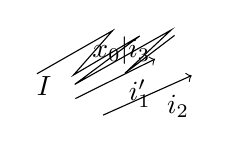
\begin{tikzpicture}[scale=.75]
\node at (0,0) {$I$};\draw[->] (.53,-.22)--(1.88,.45);\draw[->] (1,-.50)--(2.50,.17);
\node at (1.31,.59) {$\unsure{x_0|i_3}$};\node at (1.62,-.14) {$\unsure{i'_1}$};\node at (2.27,-.35) {$\unsure{i_2}$};
\draw (-.12,.2)--(1.16,.93)--(.5,.18)--(1.62,.84)--(.52,.02)--(2.15,.94)--(1.37,.21)--(2.21,.85);
\end{tikzpicture}}

% same line, to right of sketch
\deleted{Si $i\in I$, $i$ est lié à}

% ll. 9–12
$(i,\nu)$ et $(\unsure{j'|j},\mu)$ \inserted{(distincts)} sont liés ssi $i=j$ \uline{ou} $\nu=\mu$

% second condition
\[
\begin{aligned}
(i,\nu)\text{ et }(j,\pi,\rho)\quad &\deleted{\unsure{\text{sont}}}\ \text{liés }\deleted{\unsure{\text{ssi}}}\quad\text{si}\\
&\text{dans les cas }\left\{\begin{array}{ll}
i=\deleted{\unsure{j'}}j &\nu=0\\
i\ne j&\left\{\begin{array}{l}\nu=1,\ j=\rho i\\ \nu=2,\ i=\rho j\end{array}\right.
\end{array}\right.
\end{aligned}
\]

% third condition
\[
\begin{aligned}
(j,\pi,\rho)\text{ et }(j',\pi',\rho')&\ \inserted{\text{distincts}}\quad\text{liés}\\
(\underset{I}{\uparrow}\ \underset{\Pi}{\uparrow}\ \underset{\omega(I)}{\uparrow}
\qquad\text{id})&\quad\text{dans les cas }\left\{\begin{array}{ll}
j=j'&\pi=\pi',(\rho\ne\rho')\\
j\ne j'&\left\{\begin{array}{ll}i\ne j,&\rho=\rho'\\\unsure{i|i'}=j&\rho\ne\rho'\end{array}\right.
\end{array}\right.
\end{aligned}
\]

% left of three conditions
\figure{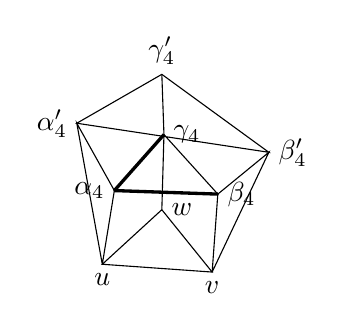
\begin{tikzpicture}[scale=.9]
\coordinate (u) at (.2,0);\coordinate (v) at (1.75,-.11);\coordinate (w) at (1.04,.77);
\coordinate (a) at (.37,1.04);\coordinate (b) at (1.83,.99);\coordinate (g) at (1.07,1.83);
\coordinate (aa) at (-.16,1.99);\coordinate (bb) at (2.55,1.58);\coordinate (gg) at (1.04,2.68);
\draw (u)--(w)--(v)--cycle (a)--(g)--(b)--cycle (aa)--(gg)--(bb)--cycle;
\draw (u)--(a)--(aa)--(u) (v)--(b)--(bb)--(v) (w)--(g)--(gg); \draw[very thick] (a)--(g) (a)--(b);
\node[below] at (u) {$u$}; \node[below] at (v) {$v$}; \node[right] at (w) {$w$};
\node[left] at (a) {$\alpha_4$}; \node[right] at (b) {$\beta_4$}; \node[right] at (g) {$\gamma_4$};
\node[left] at (aa) {$\alpha'_4$}; \node[right] at (bb) {$\beta'_4$}; \node[above] at (gg) {$\gamma'_4$};
\end{tikzpicture}}

% ll. 14–20
L'autom $\sigma$ conserve $I\times[0,1,2]$ et son complémentaire, et agit \deleted{\unsure{sur}} \unsure{en permu|sur le premier} \deleted{via} l'identité sur $I$, et la permutation entre 1 et 2 sur l'autre facteur ; sur $I\times\Pi\times\omega(I)$ il agit par permutation des deux \deleted{facteurs} élmts de $\omega(I)$ (et l'identité sur $I\times\Pi$).

% left beside action, two columns of jottings
\margin{$\underbrace{\unsure{i\,u|u}\overset{\text{ou}}{/}\alpha_4\overset{\text{ou}}{/}\alpha'_4}$ \quad $\unsure{\alpha_i},\alpha'_{\unsure{i}}$\\
$(\deleted{\unsure{u}},\underset{1\leq{i}\leq3}{\deleted{\unsure{\pi}}\pi},\rho)\ \inserted{\unsure{\alpha'_u}}$\quad $\beta_j\quad\beta'_j$\\
$1\leq i,j\leq3$\\ $\alpha_u$ ou $\alpha'_u$}

% ll. 21–22
\[
\begin{aligned}
&I\sqcup(I\times\varepsilon)\sqcup(I\times\Pi\times\varepsilon\times\omega(I)/\mathbb F_2)\\
&(I\times J)\sqcup
\end{aligned}
\]

% bottom left, crossed table
\diagram{\(\displaystyle\deleted{\begin{array}{lll}
\alpha_4&\beta_4&\gamma_4\\
\alpha'_4,&\beta'_4,&\gamma'_4,\\
\alpha_1,&\beta_2,&\gamma_3\\
\unsure{\alpha_1},&\unsure{\beta'_4},&\unsure{\gamma'_4}
\end{array}}\)}
% archive sheet number: 13
